\documentclass[a4paper,12pt]{article}
\usepackage{hyperref}
\hypersetup{
  colorlinks=true,
  linkcolor=blue,
  filecolor=magenta,
  urlcolor=cyan,
  pdftitle={Overleaf Example},
  pdfpagemode=FullScreen,
}
\usepackage[T1]{fontenc}
\usepackage{ninecolors}
\usepackage{booktabs}
\usepackage{caption}
\usepackage{tabularray}
\usepackage{geometry}
\usepackage{siunitx}
\usepackage{pdfpages}

\begin{document}
\begin{titlepage}
  \vspace*{\stretch{1.0}}
  \begin{center}
    \Large\textbf{Elements: Modulation}\\
    \large{Effect Design Workshop by Pedal Markt}
  \end{center}
  \vspace*{\fill}
  \begin{center}
    \today
  \end{center}
\end{titlepage}

\section{Summary}

Elements: Modulation is the second event in the series of
our effect-design workshops. The goal is to give you all the
tools, knowledge and a bit of intuition to start designing
effects yourself!

The workshop covers:

\begin{itemize}
  \item How modulation effects work and what parts they
    consist of;
  \item Sources, transformations and destinations that can
    we use can use CV (Control Voltage) with;
  \item Adding CV to almost any circuit.
\end{itemize}

\section{Voltage Standard}

All the workshop boards use \SI{4.5}{\V} reference voltage
as a virtual ground. Votages below \SI{4.5}{\V} are
considered negative, above \SI{4.5}{\V} --- positive.
Circuits \textit{can} accepts and output control voltage in
the range \SI{0}{\V}-\SI{9}{\V}, but an effective range is
considered to be \SI{2}{\V}-\SI{7}{\V} (\SI{5}{\V} range
centered around \SI{4.5}{\V}).

That voltage standard makes sense for effect pedals, but
some of the circuits are a bit more complex than they would
be in a triple voltage rail system like Eurorack. My
personal observation is that the world is moving on to
dual rail systems, so learning to work with them might
benefit you in any case.

\section{Included modules}

Here's a list of modules included with the worskshop and
their functions:

\begin{itemize}
  \item \textbf{AttVert} --- Two attenuverters with offset. Can
    be used as a DC voltage source or to scale and shift
    an incoming signal;

  \item \textbf{Longwave} --- LFO module based on
    \href{https://electricdruid.net/datasheets/STOMPLFODatasheet.pdf}{StompLFO}
    digital chip;

  \item \textbf{Mag} --- 2x exponential and 1x linear VCA
    module based on
    \href{https://www.soundsemiconductor.com/downloads/ssi2164datasheet.pdf}{SSI2164}
    analog 4-in-1 VCA chip;

  \item \textbf{Demod} --- Envelope follower and peak
    detector;
\end{itemize}

\pagebreak


AttVert is two attenuverters with offset function on a
single board.

\begin{itemize}
  \item Schematic PDF: \href{}{GitHub}
  \item KiCad project: \href{}{GitHub}
\end{itemize}


\begin{table}[h!]
  \caption{AttVert Pinout}
  \centerline{
    \begin{tblr}{
      hlines,
      vlines,
      rows={ht=1.2em},
      row{1}={bg=gray3,fg=white},
      colspec={cccl}
    }
      \textbf{Pin}
      & \textbf{Name}
      & \textbf{Direction}
      & \textbf{Description}
      \\
      1 & In1 & In & Input of the first attenuverter, defaults
      to \SI{4.5}{\V} when unconnected
      \\
      2 & GND & Pwr & Ground
      \\
      3 & Out1 & Out & Output of the first attenuverter
      \\
      4 & 9V0 & Pwr & \SI{9}{\V} power
      \\
      5 & GND & Pwr & Ground
      \\
      6 & 4V5 & Ref & \SI{4.5}{\V} reference
      \\
      7 & In2 & In & Input of the second attenuverter, defaults
      to \SI{4.5}{\V} when unconnected
      \\
      8 & GND & Pwr & Ground
      \\
      9 & Out2 & Out & Output of the second attenuverter
    \end{tblr}
  }
\end{table}

\pagebreak

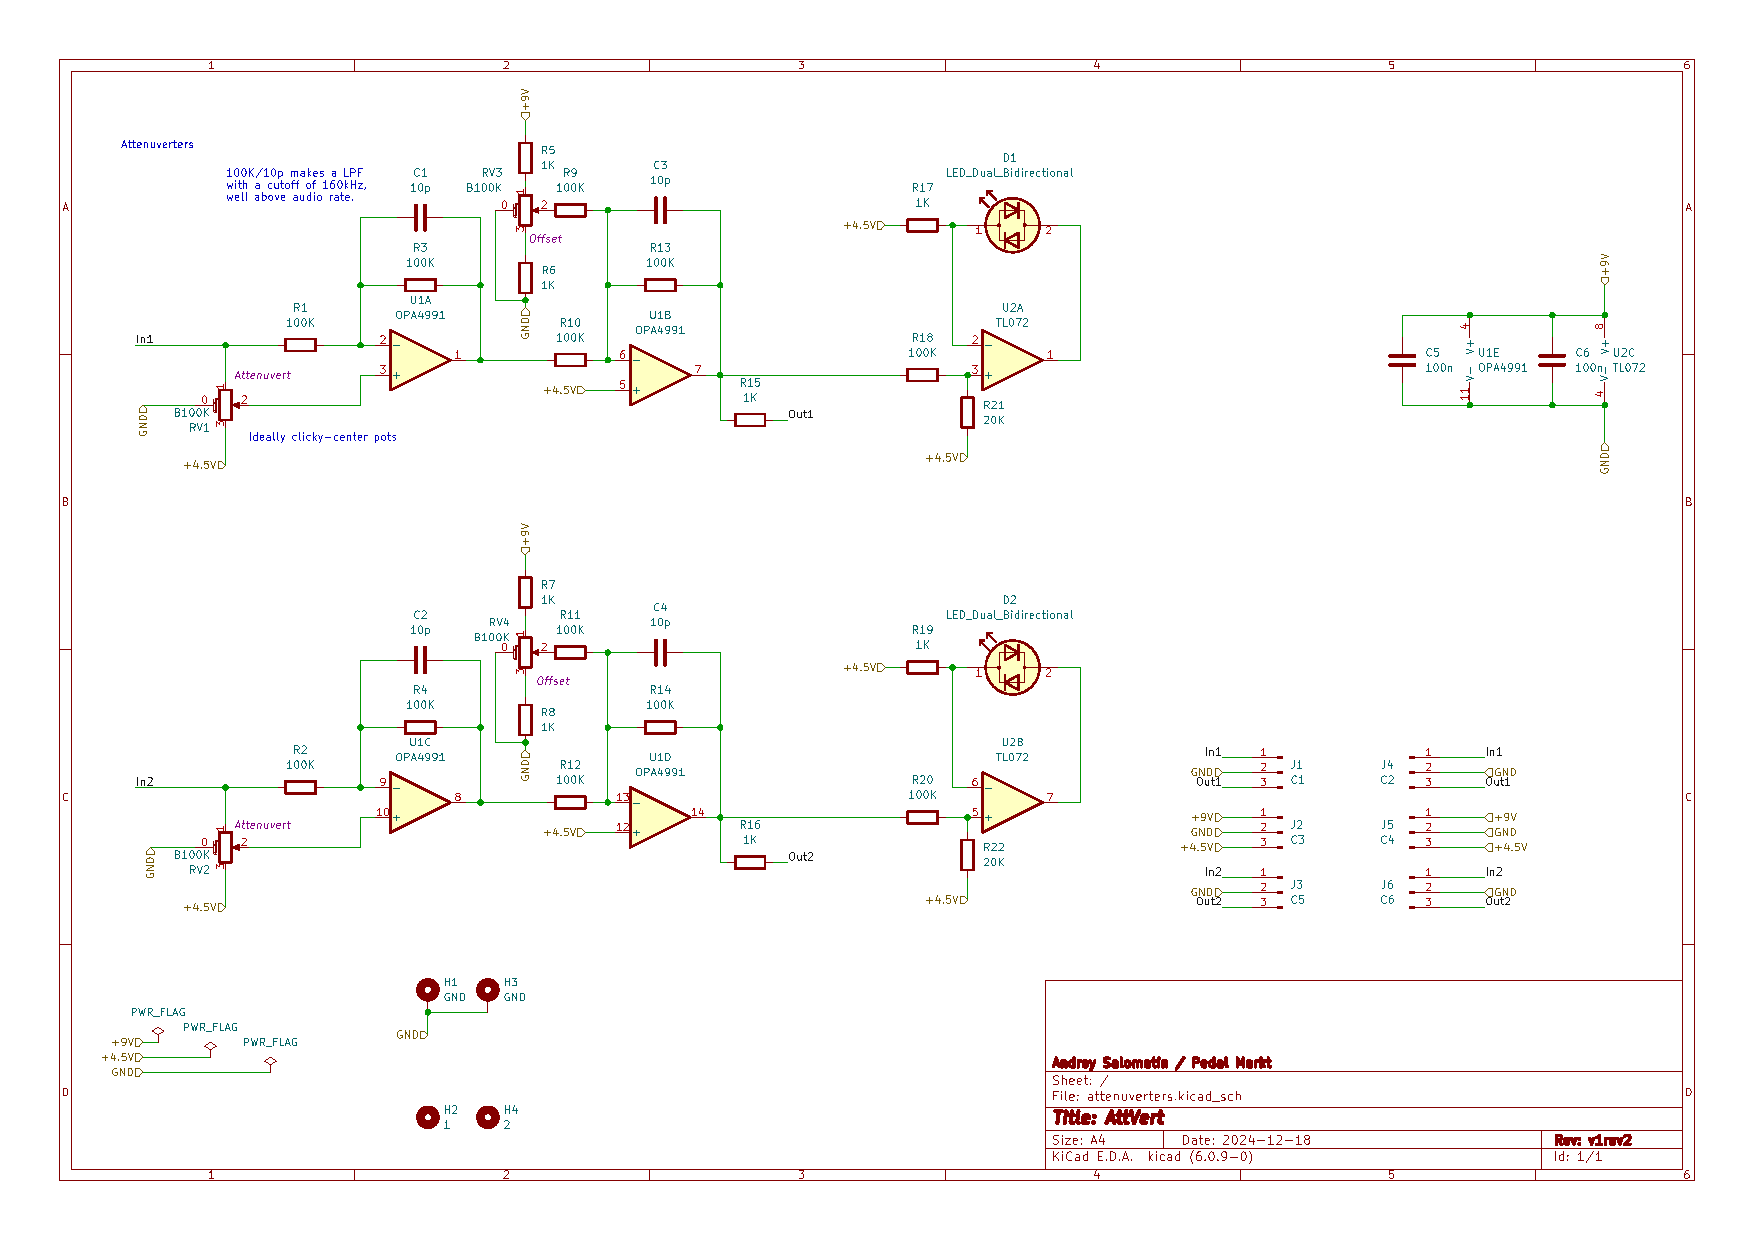
\includepdf[pages=-,landscape=true]{include/attvert-v1rev2.pdf}

\end{document}
